% Copyright (c) 2026 CorrectBrain
% SPDX-License-Identifier: MIT

\PassOptionsToPackage{dvipsnames,svgnames,x11names}{xcolor}
\documentclass[tikz,border=8pt]{standalone}
\usetikzlibrary{arrows.meta,positioning,calc,shapes,shadows,decorations.pathmorphing,shapes.geometric,backgrounds,decorations.markings,decorations.pathreplacing,decorations.text,fit,shapes.misc,shapes.arrows,matrix,bending,3d,chains,intersections,shapes.symbols,svg.path,shapes.multipart,snakes,shapes.callouts,angles,quotes}
\providecolor{gold}{RGB}{212,175,55}
\providecolor{silver}{RGB}{192,192,192}
\providecolor{bronze}{RGB}{205,127,50}
\providecolor{darkblue}{RGB}{0,0,139}
\providecolor{lightblue}{RGB}{173,216,230}
\providecolor{darkgreen}{RGB}{0,100,0}
\providecolor{lightgreen}{RGB}{144,238,144}
\providecolor{darkred}{RGB}{139,0,0}
\providecolor{navy}{RGB}{0,0,128}
\providecolor{skyblue}{RGB}{135,206,235}
\providecolor{beige}{RGB}{245,245,220}
\providecolor{cream}{RGB}{255,253,208}
\usepackage{amsmath}
\usepackage{amssymb}
\usepackage{fontawesome5}
\usetikzlibrary{fadings,shadows.blur,patterns,patterns.meta}

\providecolor{gold}{RGB}{212,175,55}
\providecolor{silver}{RGB}{192,192,192}
\providecolor{bronze}{RGB}{205,127,50}
\providecolor{darkblue}{RGB}{0,0,139}
\providecolor{lightblue}{RGB}{173,216,230}
\providecolor{darkgreen}{RGB}{0,100,0}
\providecolor{lightgreen}{RGB}{144,238,144}
\providecolor{darkred}{RGB}{139,0,0}
\providecolor{navy}{RGB}{0,0,128}
\providecolor{skyblue}{RGB}{135,206,235}
\providecolor{beige}{RGB}{245,245,220}
\providecolor{cream}{RGB}{255,253,208}
\usepackage{amsmath}
\usepackage{amssymb}
\usepackage{fontawesome5}


\providecolor{gold}{RGB}{212,175,55}
\providecolor{silver}{RGB}{192,192,192}
\providecolor{bronze}{RGB}{205,127,50}
\providecolor{darkblue}{RGB}{0,0,139}
\providecolor{lightblue}{RGB}{173,216,230}
\providecolor{darkgreen}{RGB}{0,100,0}
\providecolor{lightgreen}{RGB}{144,238,144}
\providecolor{darkred}{RGB}{139,0,0}
\providecolor{navy}{RGB}{0,0,128}
\providecolor{skyblue}{RGB}{135,206,235}
\providecolor{beige}{RGB}{245,245,220}
\providecolor{cream}{RGB}{255,253,208}
\usepackage{amsmath}
\usepackage{amssymb}
\usepackage{fontawesome5}

\usepackage{tikz}
\usepackage{xcolor}
\usepackage{helvet}
\renewcommand{\familydefault}{\sfdefault}

% --- HIGH-FIDELITY COLOR SYSTEM ---
\definecolor{csspixel}{HTML}{007ACC}       % Deep Cyan/Blue for Logical CSS
\definecolor{hwpixel}{HTML}{E74C3C}        % Crimson/Orange for Hardware Physical
\definecolor{enginecolor}{HTML}{8E44AD}    % Deep Violet/Purple for Engine Logic
\definecolor{darktext}{HTML}{2C3E50}       % High-contrast slate text
\definecolor{codebg}{HTML}{1E1E1E}         % Dark IDE code background
\definecolor{codegreen}{HTML}{A6E22E}      % Syntax highlight green
\definecolor{codeblue}{HTML}{66D9EF}       % Syntax highlight blue
\definecolor{codeyellow}{HTML}{E6DB74}     % Syntax highlight string yellow
\definecolor{subpixelred}{HTML}{FF3B30}    % Physical LED Red
\definecolor{subpixelgreen}{HTML}{34C759}  % Physical LED Green
\definecolor{subpixelblue}{HTML}{007AFF}   % Physical LED Blue
\definecolor{dotred}{HTML}{FF5F56}
\definecolor{dotyellow}{HTML}{FFBD2E}
\definecolor{dotgreen}{HTML}{27C93F}

\begin{document}
\begin{tikzpicture}[
    x=1cm, y=1cm,
    bubble/.style={
        draw=gray!30,
        fill=white,
        rounded corners=8pt,
        blur shadow={shadow opacity=16, shadow blur steps=6, shadow xshift=0.5pt, shadow yshift=-1.5pt},
        inner sep=10pt
    }
]

% --- ABSOLUTE PURE WHITE BACKGROUND ---
\fill[white] (-11.5, -14.5) rectangle (12.0863,13.5656);

% ============================================================================
% TITLE SECTION
% ============================================================================
\node[align=center, font=\Huge\bfseries, text=darktext] at (0, 12.5) {Hardware Density Grid Metrics \& \texttt{srcset}};
\node[align=center, font=\Large, text=darktext!75] at (0, 11.5) {How \texttt{1x, 2x} descriptors command the engine to map logical pixels to physical device grids.};
\draw[gray!35, line width=0.8pt] (-10, 10.5) -- (10, 10.5);

% ============================================================================
% SECTION 1: THE PIXEL GRID MAPPING (LOGICAL VS. PHYSICAL)
% ============================================================================
\node[align=center, font=\Large\bfseries, text=csspixel] at (0, 9.5) {1. The Pixel Grid Mapping (Logical vs. Physical)};

% --- Shared Isometric Basis Vectors ---
\coordinate (E1) at (1.45, 0.65);
\coordinate (E2) at (-1.45, 0.65);

% ----------------------------------------------------------------------------
% 1X CONTAINER (Standard Display) at (-7, 4.5)
% ----------------------------------------------------------------------------
\node[bubble, minimum width=6.5cm, minimum height=7.5cm] at (-7, 4.5) {};
\node[font=\large\bfseries, text=darktext] at (-7, 7.6) {Standard Display ($1x$)};
\node[font=\footnotesize, text=gray] at (-7, 7.15) {Device Pixel Ratio (DPR) = 1.0};

% Coordinates for 1x
\coordinate (O1) at (-7, 2.55);
\coordinate (T1) at (-7, 4.55);

% Hardware 3D Extrusion Side Panels (Bottom Layer)
\fill[gray!75!black] ($ (O1) + (E2) $) -- (O1) -- ($ (O1) - (0, 0.22) $) -- ($ (O1) + (E2) - (0, 0.22) $) -- cycle;
\draw[black!60, thin] ($ (O1) + (E2) $) -- (O1) -- ($ (O1) - (0, 0.22) $) -- ($ (O1) + (E2) - (0, 0.22) $) -- cycle;
\fill[gray!55!black] (O1) -- ($ (O1) + (E1) $) -- ($ (O1) + (E1) - (0, 0.22) $) -- ($ (O1) - (0, 0.22) $) -- cycle;
\draw[black!60, thin] (O1) -- ($ (O1) + (E1) $) -- ($ (O1) + (E1) - (0, 0.22) $) -- ($ (O1) - (0, 0.22) $) -- cycle;

% Hardware Top Face Base
\fill[gray!18!black] (O1) -- ($ (O1) + (E1) $) -- ($ (O1) + (E1) + (E2) $) -- ($ (O1) + (E2) $) -- cycle;
\draw[hwpixel, line width=1.4pt] (O1) -- ($ (O1) + (E1) $) -- ($ (O1) + (E1) + (E2) $) -- ($ (O1) + (E2) $) -- cycle;

% 1x RGB Subpixel LED Strips
\fill[subpixelred, draw=red!40!white, line width=0.3pt]
    ($ (O1) + 0.10*(E1) + 0.10*(E2) $) -- ($ (O1) + 0.32*(E1) + 0.10*(E2) $) --
    ($ (O1) + 0.32*(E1) + 0.90*(E2) $) -- ($ (O1) + 0.10*(E1) + 0.90*(E2) $) -- cycle;
\fill[subpixelgreen, draw=green!40!white, line width=0.3pt]
    ($ (O1) + 0.39*(E1) + 0.10*(E2) $) -- ($ (O1) + 0.61*(E1) + 0.10*(E2) $) --
    ($ (O1) + 0.61*(E1) + 0.90*(E2) $) -- ($ (O1) + 0.39*(E1) + 0.90*(E2) $) -- cycle;
\fill[subpixelblue, draw=blue!40!white, line width=0.3pt]
    ($ (O1) + 0.68*(E1) + 0.10*(E2) $) -- ($ (O1) + 0.90*(E1) + 0.10*(E2) $) --
    ($ (O1) + 0.90*(E1) + 0.90*(E2) $) -- ($ (O1) + 0.68*(E1) + 0.90*(E2) $) -- cycle;

% Vertical Projection Lines (Logical -> Hardware)
\draw[csspixel!70, dashed, thick, -Latex=3mm,] (T1) -- (O1);
\draw[csspixel!70, dashed, thick, -Latex=3mm,] ($ (T1) + (E1) $) -- ($ (O1) + (E1) $);
\draw[csspixel!70, dashed, thick, -Latex=3mm,] ($ (T1) + (E2) $) -- ($ (O1) + (E2) $);
\draw[csspixel!70, dashed, thick, -Latex=3mm,] ($ (T1) + (E1) + (E2) $) -- ($ (O1) + (E1) + (E2) $);

% Logical Layer (Top Cyan Floating Plane)
\fill[csspixel!25, fill opacity=0.55] (T1) -- ($ (T1) + (E1) $) -- ($ (T1) + (E1) + (E2) $) -- ($ (T1) + (E2) $) -- cycle;
\draw[csspixel, ultra thick] (T1) -- ($ (T1) + (E1) $) -- ($ (T1) + (E1) + (E2) $) -- ($ (T1) + (E2) $) -- cycle;
\node[font=\footnotesize\bfseries, text=csspixel!90!black, fill=white, fill opacity=0.88, text opacity=1, rounded corners=3pt, inner sep=2.5pt, draw=csspixel!40] at ($ (T1) + 0.5*(E1) + 0.5*(E2) $) {1 CSS Pixel};

% Hardware Badge & Footer Text
\node[font=\scriptsize\bfseries, text=hwpixel, fill=hwpixel!10, draw=hwpixel!40, rounded corners=3pt, inner sep=2.5pt] at (-7, 2.05) {1 Physical Pixel (RGB)};
\node[font=\footnotesize, text=darktext!80, align=center, text width=5.8cm] at (-7, 1.35) {The engine maps 1 logical unit\\to exactly 1 hardware LED/Pixel.};

% ----------------------------------------------------------------------------
% 2X CONTAINER (Retina / High-Density) at (0, 4.5)
% ----------------------------------------------------------------------------
\node[bubble, minimum width=6.5cm, minimum height=7.5cm] at (0, 4.5) {};
\node[font=\large\bfseries, text=darktext] at (0, 7.6) {Retina / High-Density ($2x$)};
\node[font=\footnotesize, text=gray] at (0, 7.15) {Device Pixel Ratio (DPR) = 2.0};

% Coordinates for 2x
\coordinate (O2) at (0, 2.55);
\coordinate (T2) at (0, 4.55);

% Hardware 3D Extrusion Side Panels
\fill[gray!75!black] ($ (O2) + (E2) $) -- (O2) -- ($ (O2) - (0, 0.22) $) -- ($ (O2) + (E2) - (0, 0.22) $) -- cycle;
\draw[black!60, thin] ($ (O2) + (E2) $) -- (O2) -- ($ (O2) - (0, 0.22) $) -- ($ (O2) + (E2) - (0, 0.22) $) -- cycle;
\fill[gray!55!black] (O2) -- ($ (O2) + (E1) $) -- ($ (O2) + (E1) - (0, 0.22) $) -- ($ (O2) - (0, 0.22) $) -- cycle;
\draw[black!60, thin] (O2) -- ($ (O2) + (E1) $) -- ($ (O2) + (E1) - (0, 0.22) $) -- ($ (O2) - (0, 0.22) $) -- cycle;

% Hardware Top Face Base
\fill[gray!18!black] (O2) -- ($ (O2) + (E1) $) -- ($ (O2) + (E1) + (E2) $) -- ($ (O2) + (E2) $) -- cycle;

% 2x2 Mini RGB Subpixels
\foreach \i in {0, 1} {
    \foreach \j in {0, 1} {
        \fill[subpixelred, draw=red!40!white, line width=0.2pt]
            ($ (O2) + {(\i*0.5 + 0.05)}*(E1) + {(\j*0.5 + 0.06)}*(E2) $) --
            ($ (O2) + {(\i*0.5 + 0.16)}*(E1) + {(\j*0.5 + 0.06)}*(E2) $) --
            ($ (O2) + {(\i*0.5 + 0.16)}*(E1) + {(\j*0.5 + 0.44)}*(E2) $) --
            ($ (O2) + {(\i*0.5 + 0.05)}*(E1) + {(\j*0.5 + 0.44)}*(E2) $) -- cycle;
        \fill[subpixelgreen, draw=green!40!white, line width=0.2pt]
            ($ (O2) + {(\i*0.5 + 0.19)}*(E1) + {(\j*0.5 + 0.06)}*(E2) $) --
            ($ (O2) + {(\i*0.5 + 0.31)}*(E1) + {(\j*0.5 + 0.06)}*(E2) $) --
            ($ (O2) + {(\i*0.5 + 0.31)}*(E1) + {(\j*0.5 + 0.44)}*(E2) $) --
            ($ (O2) + {(\i*0.5 + 0.19)}*(E1) + {(\j*0.5 + 0.44)}*(E2) $) -- cycle;
        \fill[subpixelblue, draw=blue!40!white, line width=0.2pt]
            ($ (O2) + {(\i*0.5 + 0.34)}*(E1) + {(\j*0.5 + 0.06)}*(E2) $) --
            ($ (O2) + {(\i*0.5 + 0.45)}*(E1) + {(\j*0.5 + 0.06)}*(E2) $) --
            ($ (O2) + {(\i*0.5 + 0.45)}*(E1) + {(\j*0.5 + 0.44)}*(E2) $) --
            ($ (O2) + {(\i*0.5 + 0.34)}*(E1) + {(\j*0.5 + 0.44)}*(E2) $) -- cycle;
    }
}

% 2x2 Grid Separator Lines
\draw[hwpixel, line width=1.4pt] (O2) -- ($ (O2) + (E1) $) -- ($ (O2) + (E1) + (E2) $) -- ($ (O2) + (E2) $) -- cycle;
\draw[hwpixel, thick] ($ (O2) + 0.5*(E1) $) -- ($ (O2) + 0.5*(E1) + 1.0*(E2) $);
\draw[hwpixel, thick] ($ (O2) + 0.5*(E2) $) -- ($ (O2) + 1.0*(E1) + 0.5*(E2) $);

% Styled Brace for 2x2 Hardware Grid (Realigned Vector)
\draw[decorate, decoration={brace, amplitude=4pt, mirror}, thick, hwpixel]
    ($ (O2) + (E1) + (0.35, -0.25) $) -- ($ (O2) + (0.35, -0.25) $)
    node[midway, below right=4pt, font=\tiny\bfseries, text=hwpixel] {2$\times$2 HW Grid};

% Vertical Projection Lines (Logical -> Hardware)
\draw[csspixel!70, dashed, thick, -Latex=3mm,] (T2) -- (O2);
\draw[csspixel!70, dashed, thick, -Latex=3mm,] ($ (T2) + (E1) $) -- ($ (O2) + (E1) $);
\draw[csspixel!70, dashed, thick, -Latex=3mm,] ($ (T2) + (E2) $) -- ($ (O2) + (E2) $);
\draw[csspixel!70, dashed, thick, -Latex=3mm,] ($ (T2) + (E1) + (E2) $) -- ($ (O2) + (E1) + (E2) $);

% Logical Layer (Top Cyan Floating Plane)
\fill[csspixel!25, fill opacity=0.55] (T2) -- ($ (T2) + (E1) $) -- ($ (T2) + (E1) + (E2) $) -- ($ (T2) + (E2) $) -- cycle;
\draw[csspixel, ultra thick] (T2) -- ($ (T2) + (E1) $) -- ($ (T2) + (E1) + (E2) $) -- ($ (T2) + (E2) $) -- cycle;
\node[font=\footnotesize\bfseries, text=csspixel!90!black, fill=white, fill opacity=0.88, text opacity=1, rounded corners=3pt, inner sep=2.5pt, draw=csspixel!40] at ($ (T2) + 0.5*(E1) + 0.5*(E2) $) {1 CSS Pixel};

% Hardware Badge & Footer Text
\node[font=\scriptsize\bfseries, text=hwpixel, fill=hwpixel!10, draw=hwpixel!40, rounded corners=3pt, inner sep=2.5pt] at (0, 1.75) {4 Physical Pixels (2$\times$2 Grid)};
\node[font=\footnotesize, text=darktext!80, align=center, text width=5.8cm] at (0, 1.05) {The engine divides the logical space\\into a \textbf{2x2} hardware grid (4 physical pixels).};

% ----------------------------------------------------------------------------
% 3X CONTAINER (Super High-Density) at (7, 4.5)
% ----------------------------------------------------------------------------
\node[bubble, minimum width=6.5cm, minimum height=7.5cm] at (7, 4.5) {};
\node[font=\large\bfseries, text=darktext] at (7, 7.6) {Super High-Density ($3x$)};
\node[font=\footnotesize, text=gray] at (7, 7.15) {Device Pixel Ratio (DPR) = 3.0};

% Coordinates for 3x
\coordinate (O3) at (7, 2.55);
\coordinate (T3) at (7, 4.55);

% Hardware 3D Extrusion Side Panels
\fill[gray!75!black] ($ (O3) + (E2) $) -- (O3) -- ($ (O3) - (0, 0.22) $) -- ($ (O3) + (E2) - (0, 0.22) $) -- cycle;
\draw[black!60, thin] ($ (O3) + (E2) $) -- (O3) -- ($ (O3) - (0, 0.22) $) -- ($ (O3) + (E2) - (0, 0.22) $) -- cycle;
\fill[gray!55!black] (O3) -- ($ (O3) + (E1) $) -- ($ (O3) + (E1) - (0, 0.22) $) -- ($ (O3) - (0, 0.22) $) -- cycle;
\draw[black!60, thin] (O3) -- ($ (O3) + (E1) $) -- ($ (O3) + (E1) - (0, 0.22) $) -- ($ (O3) - (0, 0.22) $) -- cycle;

% Hardware Top Face Base
\fill[gray!18!black] (O3) -- ($ (O3) + (E1) $) -- ($ (O3) + (E1) + (E2) $) -- ($ (O3) + (E2) $) -- cycle;

% 3x3 Mini RGB Subpixels
\foreach \i in {0, 1, 2} {
    \foreach \j in {0, 1, 2} {
        \fill[subpixelred, draw=red!40!white, line width=0.15pt]
            ($ (O3) + {(\i*0.3333 + 0.03)}*(E1) + {(\j*0.3333 + 0.04)}*(E2) $) --
            ($ (O3) + {(\i*0.3333 + 0.10)}*(E1) + {(\j*0.3333 + 0.04)}*(E2) $) --
            ($ (O3) + {(\i*0.3333 + 0.10)}*(E1) + {(\j*0.3333 + 0.29)}*(E2) $) --
            ($ (O3) + {(\i*0.3333 + 0.03)}*(E1) + {(\j*0.3333 + 0.29)}*(E2) $) -- cycle;
        \fill[subpixelgreen, draw=green!40!white, line width=0.15pt]
            ($ (O3) + {(\i*0.3333 + 0.13)}*(E1) + {(\j*0.3333 + 0.04)}*(E2) $) --
            ($ (O3) + {(\i*0.3333 + 0.20)}*(E1) + {(\j*0.3333 + 0.04)}*(E2) $) --
            ($ (O3) + {(\i*0.3333 + 0.20)}*(E1) + {(\j*0.3333 + 0.29)}*(E2) $) --
            ($ (O3) + {(\i*0.3333 + 0.13)}*(E1) + {(\j*0.3333 + 0.29)}*(E2) $) -- cycle;
        \fill[subpixelblue, draw=blue!40!white, line width=0.15pt]
            ($ (O3) + {(\i*0.3333 + 0.23)}*(E1) + {(\j*0.3333 + 0.04)}*(E2) $) --
            ($ (O3) + {(\i*0.3333 + 0.30)}*(E1) + {(\j*0.3333 + 0.04)}*(E2) $) --
            ($ (O3) + {(\i*0.3333 + 0.30)}*(E1) + {(\j*0.3333 + 0.29)}*(E2) $) --
            ($ (O3) + {(\i*0.3333 + 0.23)}*(E1) + {(\j*0.3333 + 0.29)}*(E2) $) -- cycle;
    }
}

% 3x3 Grid Separator Lines
\draw[hwpixel, line width=1.4pt] (O3) -- ($ (O3) + (E1) $) -- ($ (O3) + (E1) + (E2) $) -- ($ (O3) + (E2) $) -- cycle;
\draw[hwpixel, thick] ($ (O3) + 0.3333*(E1) $) -- ($ (O3) + 0.3333*(E1) + 1.0*(E2) $);
\draw[hwpixel, thick] ($ (O3) + 0.6667*(E1) $) -- ($ (O3) + 0.6667*(E1) + 1.0*(E2) $);
\draw[hwpixel, thick] ($ (O3) + 0.3333*(E2) $) -- ($ (O3) + 1.0*(E1) + 0.3333*(E2) $);
\draw[hwpixel, thick] ($ (O3) + 0.6667*(E2) $) -- ($ (O3) + 1.0*(E1) + 0.6667*(E2) $);

% Styled Brace for 3x3 Hardware Grid (Realigned Vector)
\draw[decorate, decoration={brace, amplitude=4pt, mirror}, thick, hwpixel]
    ($ (O3) + (E1) + (0.35, -0.25) $) -- ($ (O3) + (0.35, -0.25) $)
    node[midway, below right=4pt, font=\tiny\bfseries, text=hwpixel] {3$\times$3 HW Grid};

% Vertical Projection Lines (Logical -> Hardware)
\draw[csspixel!70, dashed, thick, -Latex=3mm,] (T3) -- (O3);
\draw[csspixel!70, dashed, thick, -Latex=3mm,] ($ (T3) + (E1) $) -- ($ (O3) + (E1) $);
\draw[csspixel!70, dashed, thick, -Latex=3mm,] ($ (T3) + (E2) $) -- ($ (O3) + (E2) $);
\draw[csspixel!70, dashed, thick, -Latex=3mm,] ($ (T3) + (E1) + (E2) $) -- ($ (O3) + (E1) + (E2) $);

% Logical Layer (Top Cyan Floating Plane)
\fill[csspixel!25, fill opacity=0.55] (T3) -- ($ (T3) + (E1) $) -- ($ (T3) + (E1) + (E2) $) -- ($ (T3) + (E2) $) -- cycle;
\draw[csspixel, ultra thick] (T3) -- ($ (T3) + (E1) $) -- ($ (T3) + (E1) + (E2) $) -- ($ (T3) + (E2) $) -- cycle;
\node[font=\footnotesize\bfseries, text=csspixel!90!black, fill=white, fill opacity=0.88, text opacity=1, rounded corners=3pt, inner sep=2.5pt, draw=csspixel!40] at ($ (T3) + 0.5*(E1) + 0.5*(E2) $) {1 CSS Pixel};

% Hardware Badge & Footer Text (Zero Overlap with Grid Lines)
\node[font=\scriptsize\bfseries, text=hwpixel, fill=hwpixel!10, draw=hwpixel!40, rounded corners=3pt, inner sep=2.5pt] at (7, 1.75) {9 Physical Pixels (3$\times$3 Grid)};
\node[font=\footnotesize, text=darktext!80, align=center, text width=5.8cm] at (7, 1.05) {The engine divides the logical space\\into a \textbf{3x3} hardware grid (9 physical pixels).};


% ============================================================================
% SECTION 2: THE EVALUATION PIPELINE & OS QUERY DISCONNECT
% ============================================================================
\draw[gray!35, line width=0.8pt] (-10, -0.4) -- (10, -0.4);
\node[align=center, font=\Large\bfseries, text=enginecolor] at (0, -1.0) {2. The OS Query \& Layout Disconnect};

% --- Left Module: Realistic macOS-style IDE Code Box (Strict Absolute Coordinates) ---
\fill[codebg, rounded corners=6pt, blur shadow={shadow opacity=22, shadow blur steps=6, shadow xshift=0.5pt, shadow yshift=-1.5pt}]
    (-9.5, -6.5) rectangle (-3.5, -2.5);

% IDE Title Bar with Traffic Light Dots
\fill[gray!22!black, rounded corners=6pt] (-9.5, -3.15) rectangle (-3.5, -2.5);
\fill[gray!22!black] (-9.5, -3.15) rectangle (-3.5, -2.9);
\draw[gray!35!black, line width=0.6pt] (-9.5, -3.15) -- (-3.5, -3.15);

\fill[dotred] (-9.05, -2.82) circle (3.2pt);
\fill[dotyellow] (-8.65, -2.82) circle (3.2pt);
\fill[dotgreen] (-8.25, -2.82) circle (3.2pt);
\node[font=\scriptsize\ttfamily, text=gray!60] at (-6.5, -2.82) {index.html};

% Code Syntax Highlighting
\node[anchor=north west, font=\ttfamily\small, text=white] at (-9.2, -3.3) {\textcolor{gray!60}{<}\textcolor{codeblue}{img} \textcolor{codegreen}{src}=\textcolor{codeyellow}{"logo.jpg"}};
\node[anchor=north west, font=\ttfamily\small, text=white] at (-9.2, -4.0) {\quad \textcolor{codeblue}{srcset}=\textcolor{codeyellow}{"logo-1x.jpg} \textcolor{codegreen}{1x}\textcolor{codeyellow}{,}};
\node[anchor=north west, font=\ttfamily\small, text=white] at (-9.2, -4.7) {\quad \quad \quad \quad \ \textcolor{codeyellow}{logo-2x.jpg} \textcolor{codegreen}{2x}\textcolor{codeyellow}{"}};
\node[anchor=north west, font=\ttfamily\small, text=white] at (-9.2, -5.5) {\quad \textcolor{codeblue}{width}=\textcolor{codeyellow}{"100\%"} \textcolor{gray!60}{>}};

\node[font=\footnotesize\bfseries, text=darktext!75] at (-6.5, -6.85) {\faCode\ Browser parses DOM tree};

% --- Right Module: Preload Scanner & HTML Parser Box ---
\node[bubble, minimum width=9.2cm, minimum height=4.6cm, fill=enginecolor!5, draw=enginecolor, line width=1.2pt] at (7.1, -4.0) {};

% Metallic Circuitry Pins
\foreach \y in {-3.5, -4.0, -5.0} {
    \draw[gray!60, line width=2pt] (2.2, \y) -- (2.5, \y);
    \draw[gray!60, line width=2pt] (11.7, \y) -- (12.0, \y);
}

% Engine Header
\node[font=\Large\bfseries, text=enginecolor] at (7.1, -2.2) {\faCogs\ Preload Scanner \& HTML Parser};

% Sequential Sub-Panels
\node[fill=white, draw=gray!30, rounded corners=4pt, inner sep=4.5pt, text width=7.2cm] at (7.1, -3.0) {
    \textbf{\textcolor{darktext}{Step 1:}} \ Identify density descriptors (\texttt{1x, 2x}).
};
\node[fill=white, draw=gray!30, rounded corners=4pt, inner sep=4.5pt, text width=7.2cm] at (7.1, -4.0) {
    \textbf{\textcolor{darktext}{Step 2:}} \ Query Operating System for Hardware DPR.
};
\node[fill=hwpixel!10, draw=hwpixel!50, rounded corners=4pt, inner sep=4.5pt, text width=7.2cm] at (7.1164,-5.46) {
    \textbf{\textcolor{hwpixel}{Step 3:}} \ \textcolor{hwpixel}{\textbf{Ignore CSS Layout entirely.}} Download match.
};

% --- Center Module: OS Kernel Module ---
\node[draw=darktext!60, fill=gray!10, rounded corners=5pt, inner sep=4.5pt, blur shadow={shadow opacity=16, shadow blur steps=4}, align=center, minimum width=4.5cm, minimum height=1.2cm] (oskernel) at (0, -6.2) {
    \faMicrochip\ \textbf{OS Kernel / Display Driver}\\
    \scriptsize \texttt{window.devicePixelRatio = 2.0}
};

% --- Logical Node (CSSOM Layout Phase - Evaluated Later) ---
\node[fill=gray!5, draw=gray!40, dashed, rounded corners=4pt, inner sep=4.5pt, text width=7.2cm, align=center] (cssom) at (7.1, -8.0) {
    \textbf{\textcolor{gray}{\faPaintBrush\ CSSOM Layout Engine}} \textcolor{gray}{(Evaluated Later)}
};

% --- Orthogonal Logic Routing (Zero Overlap Arrow Paths) ---

% Arrow 1 (Parsed Tag)
\draw[-Latex, line width=2pt, enginecolor!80!black] (-3.5, -3.5) -- (2.5, -3.5);
\node[font=\scriptsize\bfseries, text=enginecolor!80!black, fill=white, inner sep=2pt] at (-0.5, -3.25) {Parsed Tag};

% Arrow 2 (Query DPR)
\draw[-Latex, dashed, thick, darktext!70] (2.5, -4.0) -- (1.0, -4.0) -- ([xshift=1cm]oskernel.north);
\node[font=\tiny\bfseries, text=darktext, fill=white, inner sep=2pt] at (1.7828,-3.8815) {Query DPR};

% Arrow 3 (Hardware DPR Data)
\draw[-Latex, very thick, hwpixel] ([xshift=-1cm]oskernel.north) -- (-1.0, -5.0) -- (2.5, -5.0);
\node[font=\tiny\bfseries, text=hwpixel, fill=white, inner sep=2pt] at (0.0603,-4.7664) {Hardware DPR Data};

% Arrow 4 (The Ignored CSS Disconnect - Critical Fix)
\node[fill=white, draw=hwpixel, rounded corners=3pt, inner sep=4.5pt, font=\scriptsize\bfseries, text=hwpixel] (ignorebadge) at (0, -8.0) {\faTimes\ Ignored during Preload};
\draw[dashed, thick, gray!60] (-3.5, -5.8) -- (-2.8941,-5.8164) -- (-2.8941,-8.0164) -- (ignorebadge.west);
\draw[-Latex, dashed, thick, gray!60] (ignorebadge.east) -- (cssom.west);


% ============================================================================
% SECTION 3: THE ABSOLUTE RULE (STRICT HARDWARE COMMAND)
% ============================================================================
\node[bubble, minimum width=17.0cm, minimum height=2.8cm, fill=hwpixel!5, draw=hwpixel!60, line width=1pt] at (0, -11.5) {};

% Bold Red Accent Left-Border
\draw[hwpixel, line width=4.5pt, line cap=round] (-8.3, -10.3) -- (-8.3, -12.7);

% Custom High-Fidelity Warning Sign (Micro-aligned Centroid)
\fill[yellow!90!orange, draw=black!85, line width=1.4pt, line join=round]
    (-7.3, -10.85) -- (-7.9, -12.05) -- (-6.7, -12.05) -- cycle;
\node[font=\bfseries\Large, text=black] at (-7.3, -11.45) {!};

% Panel Title & Explanatory Copy
\node[font=\Large\bfseries, text=hwpixel, anchor=west] at (-6.1, -10.65) {Strict Hardware Command (The Absolute Rule)};
\node[font=\normalsize, text=darktext, align=left, text width=14.0cm, anchor=north west] at (-6.1, -11.05) {
    When \texttt{1x, 2x} modifiers are used, the browser makes the download decision based \textbf{solely on the OS hardware metrics}. The fluid CSS layout (e.g., \texttt{width: 100\%} or \texttt{50vw}) is evaluated \textbf{after} the image source is selected, meaning responsive fluid widths cannot influence density descriptor logic.
};

\end{tikzpicture}
\end{document}
